\documentclass[12pt, titlepage]{article}

\usepackage{fullpage}
\usepackage[round]{natbib}
\usepackage{multirow}
\usepackage{booktabs}
\usepackage{tabularx}
\usepackage{graphicx}
\usepackage{float}
\usepackage{hyperref}
\hypersetup{
    colorlinks,
    citecolor=black,
    filecolor=black,
    linkcolor=red,
    urlcolor=blue
}
\usepackage[round]{natbib}

\newcounter{acnum}
\newcommand{\actheacnum}{AC\theacnum}
\newcommand{\acref}[1]{AC\ref{#1}}

\newcounter{ucnum}
\newcommand{\uctheucnum}{UC\theucnum}
\newcommand{\uref}[1]{UC\ref{#1}}

\newcounter{mnum}
\newcommand{\mthemnum}{M\themnum}
\newcommand{\mref}[1]{M\ref{#1}}

\topmargin=-0.5in
\textheight=9.5in
\oddsidemargin=-0.5in
\textwidth=7.5in

\title{SE 3XA3: Software Requirements\\Spann}

\author{Team 5
		\\ Christopher Stokes | stokescd
		\\ Varun Hooda | hoodav
}

\date{\today}

%% Comments

\usepackage{color}

\newif\ifcomments\commentstrue

\ifcomments
\newcommand{\authornote}[3]{\textcolor{#1}{[#3 ---#2]}}
\newcommand{\todo}[1]{\textcolor{red}{[TODO: #1]}}
\else
\newcommand{\authornote}[3]{}
\newcommand{\todo}[1]{}
\fi

\newcommand{\wss}[1]{\authornote{blue}{SS}{#1}}
\newcommand{\ds}[1]{\authornote{red}{DS}{#1}}
\newcommand{\mj}[1]{\authornote{red}{MSN}{#1}}
\newcommand{\cm}[1]{\authornote{red}{CM}{#1}}
\newcommand{\mh}[1]{\authornote{red}{MH}{#1}}

% team members should be added for each team, like the following
% all comments left by the TAs or the instructor should be addressed
% by a corresponding comment from the Team

\newcommand{\tm}[1]{\authornote{magenta}{Team}{#1}}


\begin{document}

\maketitle

\pagenumbering{roman}
\tableofcontents
\listoftables
\listoffigures

\begin{table}[bp]
\caption{\bf Revision History}
\begin{tabularx}{\textwidth}{p{3cm}p{2cm}X}
\toprule {\bf Date} & {\bf Version} & {\bf Notes}\\
\midrule
  Nov 10, 2016 & 1.0 & Initial Changes\\
  Nov 12, 2016 & 1.1 & Changes and Module Hierarchy\\
\bottomrule
\end{tabularx}
\end{table}

\newpage

\pagenumbering{arabic}

\section{Introduction}

Decomposing a system into modules is a commonly accepted approach to developing
software.  A module is a work assignment for a programmer or programming
team~\citep{ParnasEtAl1984}.  We advocate a decomposition
based on the principle of information hiding~\citep{Parnas1972a}.  This
principle supports design for change, because the ``secrets'' that each module
hides represent likely future changes.  Design for change is valuable in SC,
where modifications are frequent, especially during initial development as the
solution space is explored.

Our design follows the rules layed out by \citet{ParnasEtAl1984}, as follows:
\begin{itemize}
\item System details that are likely to change independently should be the
  secrets of separate modules.
\item Each data structure is used in only one module.
\item Any other program that requires information stored in a module's data
  structures must obtain it by calling access programs belonging to that module.
\end{itemize}

After completing the first stage of the design, the Software Requirements
Specification (SRS), the Module Guide (MG) is developed~\citep{ParnasEtAl1984}. The MG
specifies the modular structure of the system and is intended to allow both
designers and maintainers to easily identify the parts of the software.  The
potential readers of this document are as follows:

\begin{itemize}
\item New project members: This document can be a guide for a new project member
  to easily understand the overall structure and quickly find the
  relevant modules they are searching for.
\item Maintainers: The hierarchical structure of the module guide improves the
  maintainers' understanding when they need to make changes to the system. It is
  important for a maintainer to update the relevant sections of the document
  after changes have been made.
\item Designers: Once the module guide has been written, it can be used to
  check for consistency, feasibility and flexibility. Designers can verify the
  system in various ways, such as consistency among modules, feasibility of the
  decomposition, and flexibility of the design.
\end{itemize}

The rest of the document is organized as follows. Section
\ref{SecChange} lists the anticipated and unlikely changes of the software
requirements. Section \ref{SecMH} summarizes the module decomposition that
was constructed according to the likely changes. Section \ref{SecConnection}
specifies the connections between the software requirements and the
modules. Section \ref{SecMD} gives a detailed description of the
modules. Section \ref{SecTM} includes two traceability matrices. One checks
the completeness of the design against the requirements provided in the SRS. The
other shows the relation between anticipated changes and the modules. Section
\ref{SecUse} describes the use relation between modules.

\section{Anticipated and Unlikely Changes} \label{SecChange}

This section lists possible changes to the system. According to the likeliness
of the change, the possible changes are classified into two
categories. Anticipated changes are listed in Section \ref{SecAchange}, and
unlikely changes are listed in Section \ref{SecUchange}.

\subsection{Anticipated Changes} \label{SecAchange}

Anticipated changes are the source of the information that is to be hidden
inside the modules. Ideally, changing one of the anticipated changes will only
require changing the one module that hides the associated decision. The approach
adapted here is called design for
change.

\begin{description}
\item[\refstepcounter{acnum} \actheacnum \label{acUILooks}:] User interface
  styling (CSS).

\item[\refstepcounter{acnum} \actheacnum \label{acUILooks}:] User interface
  layout (CSS/JavaScript).

\item[\refstepcounter{acnum} \actheacnum \label{acUILooks}:] User
    Session/Authentication

\item[\refstepcounter{acnum} \actheacnum \label{acUILooks}:] Addition or
    Deletion of UI Components
\end{description}

\subsection{Unlikely Changes} \label{SecUchange}

The module design should be as general as possible. However, a general system is
more complex. Sometimes this complexity is not necessary. Fixing some design
decisions at the system architecture stage can simplify the software design. If
these decision should later need to be changed, then many parts of the design
will potentially need to be modified. Hence, it is not intended that these
decisions will be changed.

\begin{description}
    \item[\refstepcounter{ucnum} \uctheucnum \label{ucIO}:] Application
        platform (web browser)

    \item[\refstepcounter{ucnum} \uctheucnum \label{ucIO}:] Web front end
        framework

    \item[\refstepcounter{ucnum} \uctheucnum \label{ucIO}:] Web server and
        server framework

    \item[\refstepcounter{ucnum} \uctheucnum \label{ucIO}:] Database (SQL and
        PostgreSQL)
\end{description}

\section{Module Hierarchy} \label{SecMH}

This section provides an overview of the module design. Modules are summarized
in a hierarchy decomposed by secrets in Table \ref{TblMH}. The modules listed
below, which are leaves in the hierarchy tree, are the modules that will
actually be implemented.

\begin{description}
\item [\refstepcounter{mnum} \mthemnum \label{mHH}:] Hardware-Hiding Module
\item [\refstepcounter{mnum} \mthemnum \label{mHH}:] API Controllers
\item [\refstepcounter{mnum} \mthemnum \label{mHH}:] Python Console
\item [\refstepcounter{mnum} \mthemnum \label{mHH}:] Python Console Manager
\item [\refstepcounter{mnum} \mthemnum \label{mHH}:] Python Runners
\item [\refstepcounter{mnum} \mthemnum \label{mHH}:] Repository Model
\item [\refstepcounter{mnum} \mthemnum \label{mHH}:] Domain Models
\item [\refstepcounter{mnum} \mthemnum \label{mHH}:] UI Screens
\end{description}

Note: Since this system utilizes libraries and frameworks to abstract away the
low level implementation details of browser interaction, operating system
interaction and networking hardware interaction, there is(are) no
Hardware-Hiding Module(s).

%\newpage
\begin{table}[h!]
\centering
\begin{tabular}{p{0.3\textwidth} p{0.3\textwidth} p{0.3\textwidth}}
\toprule
    \textbf{Level 1} & \textbf{Level 2} &\ \textbf{Level 3}\\
\midrule

{Hardware-Hiding Module} & ~ \\
\midrule

\multirow{7}{0.3\textwidth}{
    Behaviour-Hiding Module} & API Controllers & Console Controller\\
    & -- & Fiddle Controller\\
    & -- & File Controller\\
    & -- & Project Controller\\
    & -- & User Controller\\

    & Python Console & --\\
    & Python Console Manager & --\\

    & UI Screens & App\\
    & -- & Full Screen Frame\\
    & -- & Project Frame\\
    & -- & Selection Frame\\
    & -- & Account\\
    & -- & Console\\
    & -- & Dock Screen Output\\
    & -- & Screen Fiddle\\
    & -- & Dialog Menu\\
    & -- & Editor\\
    & -- & Home\\
    & -- & Login\\
    & -- & Login State Manager\\
    & -- & Project Dialog\\
    & -- & Project Dialog State Manager\\
    & -- & Project Edit\\
    & -- & Project Transform\\
    & & \\
\bottomrule
    & Table continues on next page & \\
%     & -- & Project Edit State Manager\\
%     & -- & Project Transform\\
%     & -- & Projects\\
\end{tabular}
\end{table}

\begin{table}[h!]
\centering
\begin{tabular}{p{0.3\textwidth} p{0.3\textwidth} p{0.3\textwidth}}
\toprule
    \textbf{Level 1} & \textbf{Level 2} &\ \textbf{Level 3}\\
\midrule
    \multirow{3}{0.3\textwidth}{Software Decision Module} & Domain Models & Python File Data Transfer Object\\
    & -- & Python Project Data Transfer Object\\
    & -- & User Data Transfer Object\\
    & -- & Base Data Transfer Object\\
    & -- & Message Data Model\\
    & -- & Python File Data Model\\
    & -- & Python Project Data Model\\
    & -- & User Data Model\\
    & Repository Model & --\\
    & Python Runners & Iron Python Location\\
    & -- & Python File\\
    & -- & Python Project\\
    & -- & Python Project Manager\\
    & -- & Python Runner\\
    & -- & Python Server Manager\\
    & -- & Python Tools\\
    & -- & Iron Python Manager\\
    & -- & Notification Stream Writer\\
\bottomrule
\end{tabular}
\caption{Module Hierarchy}
\label{TblMH}
\end{table}

\section{Connection Between Requirements and Design} \label{SecConnection}

The design of the system is intended to satisfy the requirements developed in
the SRS. In this stage, the system is decomposed into modules. The connection
between requirements and modules is listed in Table \ref{TblRT}.

\section{Module Decomposition} \label{SecMD}

% Modules are decomposed according to the principle of ``information hiding''
% proposed by \citet{ParnasEtAl1984}. The \emph{Secrets} field in a module
% decomposition is a brief statement of the design decision hidden by the
% module. The \emph{Services} field specifies \emph{what} the module will do
% without documenting \emph{how} to do it. For each module, a suggestion for the
% implementing software is given under the \emph{Implemented By} title. If the
% entry is \emph{OS}, this means that the module is provided by the operating
% system or by standard programming language libraries.  Also indicate if the
% module will be implemented specifically for the software.

% Only the leaf modules in the
% hierarchy have to be implemented. If a dash (\emph{--}) is shown, this means
% that the module is not a leaf and will not have to be implemented. Whether or
% not this module is implemented depends on the programming language
% selected.

\subsection{Hardware Hiding Modules}

\begin{description}
\item[Secrets:] Networking functionality and CSS/HTML/JavaScript rendering and
    execution.
\item[Services:]Networking serves as the backbone of the API, servicing web
    requests. The web browser provides a platform for rendering website content
    and execution JavaScript code.
\item[Implemented By:] ASP.NET, Web Browsers
\end{description}

\subsection{Behaviour-Hiding Module}

\subsubsection{API Controllers}

\begin{description}
\item[Secrets:] API request handling and routing.
\item[Services:] Accept and respond to API calls from the network. Provide an
    interface with the rest of the server.
\item[Implemented By:] --
\end{description}

\subsubsection{Console Controller}

\begin{description}
\item[Secrets:] API request handling and routing for the console.
\item[Services:] Handles API requests related to the python code execution on
    the console.
\item[Implemented By:] Spann
\end{description}

\subsubsection{Fiddle Controller}

\begin{description}
\item[Secrets:] API request handling and routing for the fiddle.
\item[Services:] Handles API requests related to the fiddle code execution.
\item[Implemented By:] Spann
\end{description}

\subsubsection{File Controller}

\begin{description}
\item[Secrets:] API request handling and routing for files.
\item[Services:] Handles API requests related to source code files.
\item[Implemented By:] Spann
\end{description}

\subsubsection{Project Controller}

\begin{description}
\item[Secrets:] API request handling and routing for projects.
\item[Services:] Handles API requests related to projects.
\item[Implemented By:] Spann
\end{description}

\subsubsection{User Controller}

\begin{description}
\item[Secrets:] API request handling and routing for users and user data.
\item[Services:] Handles API request related to users, sessions and user data.
\item[Implemented By:] Spann
\end{description}



\subsubsection{Python Console}

\begin{description}
    \item[Secrets:] Handles code execution for the client (front end).
\item[Services:] Takes in a string of code and uses standard library functions
    to execute the code with a python interpreter and returns result.
\item[Implemented By:] Spann
\end{description}

\subsubsection{Python Console Manager}

\begin{description}
\item[Secrets:] Manges python consoles.
\item[Services:] Provides a support for managing multiple consoles.
\item[Implemented By:] Spann
\end{description}

\subsubsection{UI Screens}

\begin{description}
\item[Secrets:] UI layout and functionality.
\item[Services:] Provides a way of dynamically generating the UI and managing
    all the functionality of the UI.
\item[Implemented By:] --
\end{description}

\subsubsection{App}

\begin{description}
\item[Secrets:] Base application screen.
\item[Services:] Provides the base for application screens.
\item[Implemented By:] Spann
\end{description}

\subsubsection{Full Screen Frame}

\begin{description}
\item[Secrets:] Full screen UI frame component.
\item[Services:] Provides a full screen UI frame for embedding components.
\item[Implemented By:] Spann
\end{description}

\subsubsection{Project Frame}

\begin{description}
\item[Secrets:] Project frame component.
\item[Services:] Provides a frame for embedding project UI components.
\item[Implemented By:] Spann
\end{description}

\subsubsection{Selection Frame}

\begin{description}
\item[Secrets:] Selection frame component.
\item[Services:] Provides a frame for embedding selection UI components.
\item[Implemented By:] Spann
\end{description}

\subsubsection{Account}

\begin{description}
\item[Secrets:] Screen for user account.
\item[Services:] Provides a screen for displaying user account and settings.
\item[Implemented By:] Spann
\end{description}

\subsubsection{Console}

\begin{description}
\item[Secrets:] Screen for python console.
\item[Services:] Provides a screen for displaying a console for writing code
    in a interactive console mode.
\item[Implemented By:] Spann
\end{description}

\subsubsection{Dock Screen Output}

\begin{description}
\item[Secrets:] Dock screen for output.
\item[Services:] Provides a dockable screen that can be used to display output
    of a python program.
\item[Implemented By:] Spann
\end{description}

\subsubsection{Screen Fiddle}

\begin{description}
\item[Secrets:] Screen for fiddle.
\item[Services:] Provides a screen for fiddle mode (interactive console without
    signing in).
\item[Implemented By:] Spann
\end{description}

\subsubsection{Dialog Menu}

\begin{description}
\item[Secrets:] Dialog for a popup menu.
\item[Services:] Provides a popup type menu for embedding other UI components.
\item[Implemented By:] Spann
\end{description}

\subsubsection{Editor}

\begin{description}
\item[Secrets:] Screen for code editor.
\item[Services:] Provides a screen for editing python code.
\item[Implemented By:] Spann
\end{description}

\subsubsection{Home}

\begin{description}
\item[Secrets:] Home screen.
\item[Services:] Provides a home screen for when users first login.
\item[Implemented By:] Spann
\end{description}

\subsubsection{Login}

\begin{description}
\item[Secrets:] Login screen.
\item[Services:] Provides a login screen with input and buttons for users to login,
    signup or go to the fiddle.
\item[Implemented By:] Spann
\end{description}

\subsubsection{Login State Manager}

\begin{description}
\item[Secrets:] Manager for login state.
\item[Services:] Provides a manager for keeping track of logins.
\item[Implemented By:] Spann
\end{description}

\subsubsection{Project Dialog}

\begin{description}
\item[Secrets:] Project dialog component.
\item[Services:] Provides a dialog for managing project and project details.
\item[Implemented By:] Spann
\end{description}

\subsubsection{Project Dialog State Manager}

\begin{description}
\item[Secrets:] State Manager for project dialog.
\item[Services:] Provides a manager that keeps track of the project dialog's state.
\item[Implemented By:] Spann
\end{description}

\subsubsection{Project Edit}

\begin{description}
\item[Secrets:] Project editing screen.
\item[Services:] Provides a screen for managing, creating and editing projects.
\item[Implemented By:] Spann
\end{description}

\subsubsection{Project Transform}

\begin{description}
\item[Secrets:] Project transform component.
\item[Services:] Provides a project transform tree type component.
\item[Implemented By:] Spann
\end{description}



\subsection{Software Decision Module}

\subsubsection{Domain Models}

\begin{description}
\item[Secrets:] Models the data for different objects used throughout the
    application.
\item[Services:] Provides a way to model objects and hold data.
\item[Implemented By:] --
\end{description}

\subsubsection{Python File Data Transfer Object}

\begin{description}
\item[Secrets:] Model python files.
\item[Services:] A way to model python files that are transferred to the front
    end.
\item[Implemented By:] Spann
\end{description}

\subsubsection{Python Project Data Transfer Object}

\begin{description}
\item[Secrets:] Model python projects.
\item[Services:] A way to model python projects that are transferred to the front
    end.
\item[Implemented By:] Spann
\end{description}

\subsubsection{User Data Transfer Object}

\begin{description}
\item[Secrets:] Model users.
\item[Services:] A way to model user data that will be transferred to the front
    end.
\item[Implemented By:] Spann
\end{description}

\subsubsection{Base Data Transfer Object}

\begin{description}
\item[Secrets:] Base for other data transfer objects to model off.
\item[Services:] A way to provide a base class for extending other data
    transfer object classes.
\item[Implemented By:] Spann.
\end{description}

\subsubsection{Message Data Model}

\begin{description}
\item[Secrets:] Model message data.
\item[Services:] Provides a way to model messages and message data that will be
    transferred to the front end.
\item[Implemented By:] Spann
\end{description}

\subsubsection{Python File Data Model}

\begin{description}
\item[Secrets:] Model python file data.
\item[Services:] Provides a way to model python file data that will be transferred to the front end.
\item[Implemented By:] Spann
\end{description}

\subsubsection{Python Project Data Model}

\begin{description}
\item[Secrets:] Model python project data.
\item[Services:] Provides a way to model python project data that will be transferred to the front end.
\item[Implemented By:] Spann
\end{description}

\subsubsection{User Data Model}

\begin{description}
\item[Secrets:] Model user data.
\item[Services:] Provides a way to model user data that will be transferred to the front end.
\item[Implemented By:] Spann
\end{description}


\subsubsection{Repository Model}

\begin{description}
\item[Secrets:] Model repository and repository data.
\item[Services:] Provides a way to model repository that will be used by the
    application during runtime to handle different manager.
\item[Implemented By:] Spann
\end{description}

\subsubsection{Python Runners}

\begin{description}
\item[Secrets:] Python functions for various python execution tasks.
\item[Services:] Provides python functions to aid in managing python execution.
\item[Implemented By:] --
\end{description}

\subsubsection{Iron Python Location}

\begin{description}
\item[Secrets:] Iron Python Runtime location.
\item[Services:] Provides the interface to the Iron Python Runtime.
\item[Implemented By:] Spann
\end{description}

\subsubsection{Python File}

\begin{description}
\item[Secrets:] Python file object.
\item[Services:] Provides a data structure and methods for python files.
\item[Implemented By:] Spann
\end{description}

\subsubsection{Python Project}

\begin{description}
\item[Secrets:] Python project object.
\item[Services:] Provides a data structure and methods for python projects.
\item[Implemented By:] Spann
\end{description}

\subsubsection{Python Project Manager}

\begin{description}
\item[Secrets:] Python project manager object.
\item[Services:] Provides a data structure and methods for python project manager.
\item[Implemented By:] Spann
\end{description}

\subsubsection{Python Runner}

\begin{description}
\item[Secrets:] Python runner for executing python source code and whole projects.
\item[Services:] Provides an interface for launching python code or projects.
\item[Implemented By:] Spann
\end{description}


\subsubsection{Python Server Manager}

\begin{description}
\item[Secrets:] Python server manager object.
\item[Services:] Provides functionality for managing python execution.
\item[Implemented By:] Spann
\end{description}


\subsubsection{Python Tools}

\begin{description}
\item[Secrets:] Manages various python tools.
\item[Services:] Provides various python related tools for use by other components.
\item[Implemented By:] Spann
\end{description}


\subsubsection{Iron Python Manager}

\begin{description}
\item[Secrets:] Manages the Iron Python runtime.
\item[Services:] Provides an interface to manage the Iron Python Runtime.
\item[Implemented By:] Spann
\end{description}

\subsubsection{Notification Stream Writer}

\begin{description}
\item[Secrets:] Write a notification to a stream.
\item[Services:] Provides notification writing functionality when communicating
    with the front end.
\item[Implemented By:] Spann
\end{description}

\section{Traceability Matrix} \label{SecTM}

This section shows two traceability matrices: between the modules and the
requirements and between the modules and the anticipated changes.

% the table should use mref, the requirements should be named, use something
% like fref
\begin{table}[H]
\centering
\begin{tabular}{p{0.3\textwidth} p{0.4\textwidth}}
\toprule
\textbf{Req.} & \textbf{Modules}\\
\midrule
    Mode & M2, M8\\
    Editing & M2, M3, M5, M6, M7, M8\\
    Editing Support & M3, M8\\
    Refactoring & M3, M8\\
    File Handling & M2, M5, M6, M7, M8\\
    Code Execution & M2, M3, M4, M5\\
    Shell Interpreter & M2, M3, M4, M5, M8\\
    Networking & M1, M2, M8\\
    Accounts & M2, M6, M7, M8\\
    Account Management & M2, M6, M7, M8\\
    Look and Feel & M8\\
    Usability & M8\\
    Performance & M1, M4, M8\\
    Power Usage & M1\\
    Security & M2, M6, M7, M8\\
    Health and Safety & M8\\
\bottomrule
\end{tabular}
\caption{Trace Between Requirements and Modules}
\label{TblRT}
\end{table}

\begin{table}[H]
\centering
\begin{tabular}{p{0.3\textwidth} p{0.4\textwidth}}
\toprule
\textbf{AC} & \textbf{Modules}\\
\midrule
    AC1 & M8\\
    AC2 & M8\\
    AC3 & M2, M6, M7\\
    AC4 & M8\\
\bottomrule
\end{tabular}
\caption{Trace Between Anticipated Changes and Modules}
\label{TblACT}
\end{table}

\section{Use Hierarchy Between Modules} \label{SecUse}

In this section, the uses hierarchy between modules is
provided. \citet{Parnas1978} said of two programs A and B that A {\em uses} B if
correct execution of B may be necessary for A to complete the task described in
its specification. That is, A {\em uses} B if there exist situations in which
the correct functioning of A depends upon the availability of a correct

The following two figures outline the hierarchy of the modules for this
application.  Figure 1 provides the hierarchy for the server and Figure 2
provides the hierarchy for the front end UI modules.

\begin{figure}[H]
\centering
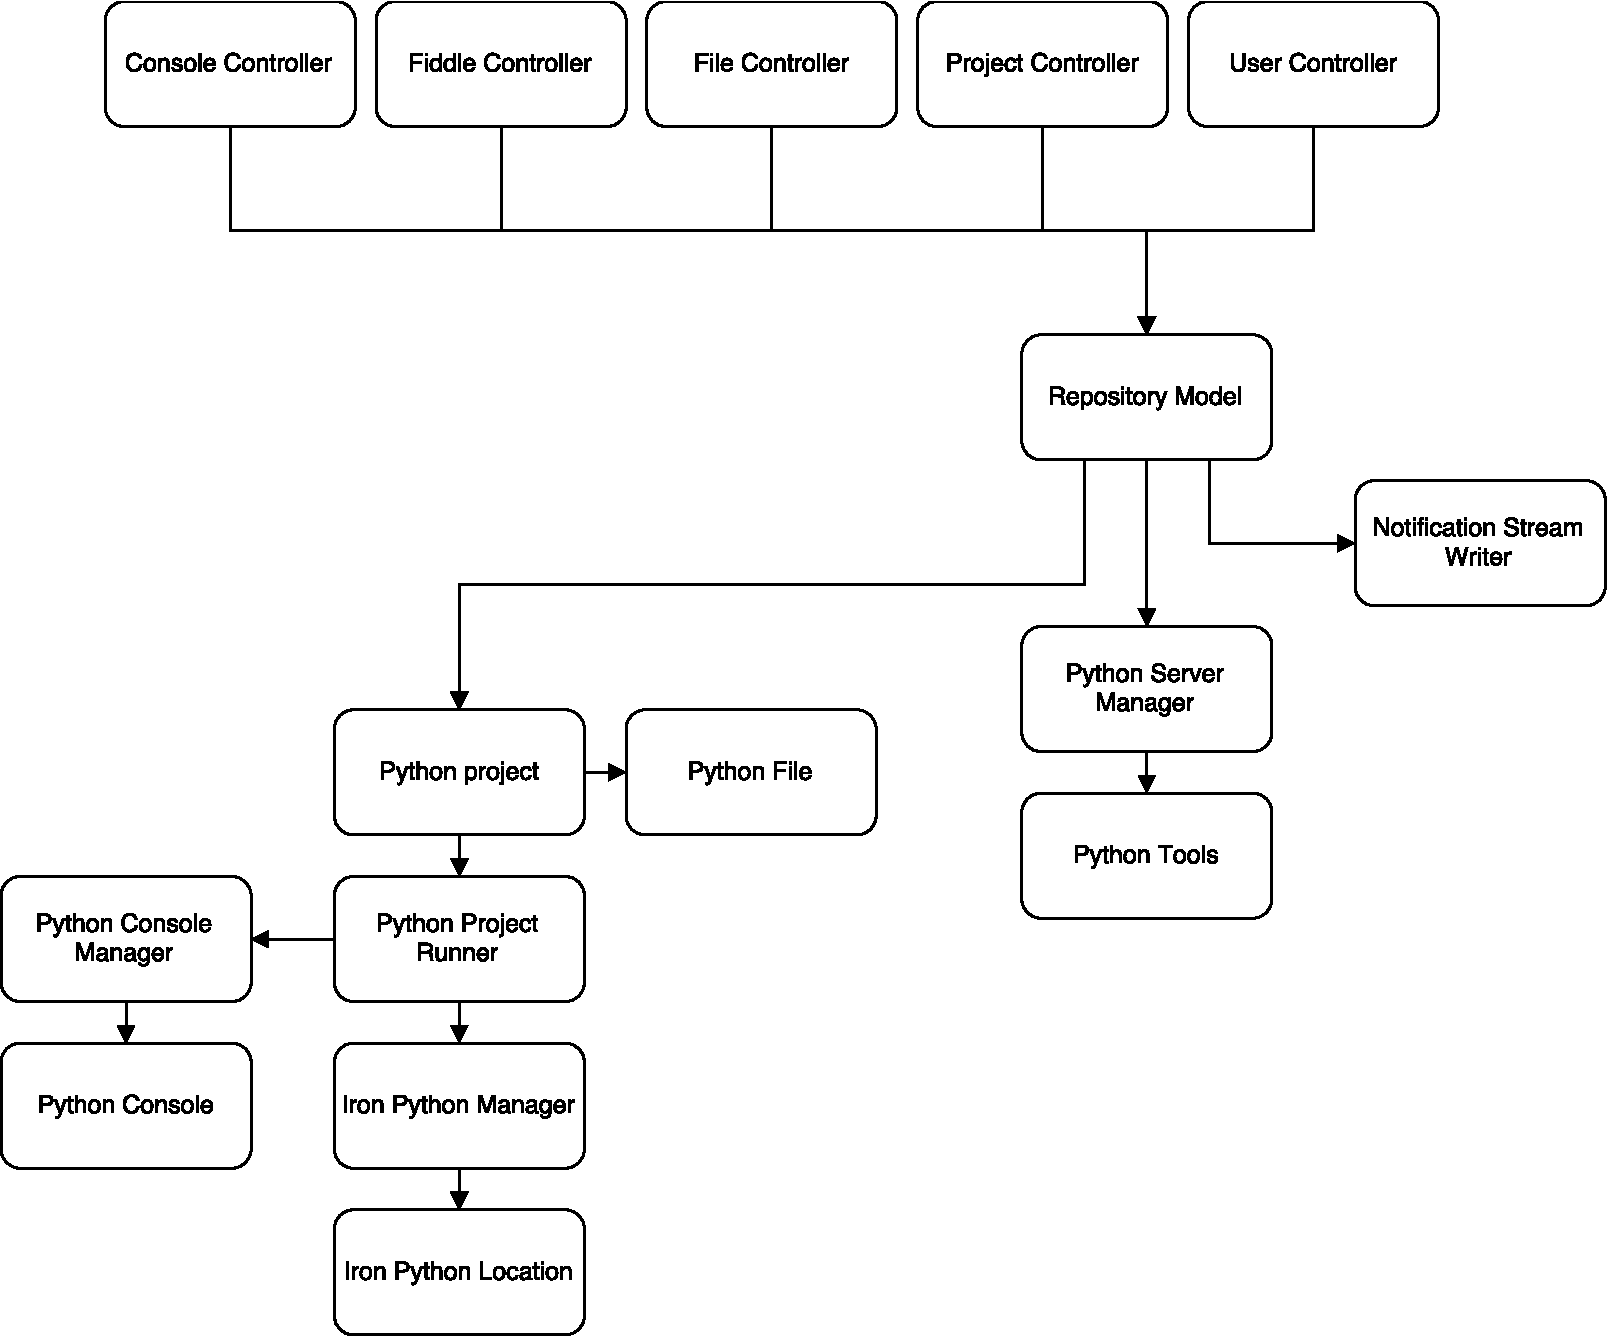
\includegraphics[width=0.7\textwidth]{uses-server.pdf}
\caption{Use hierarchy among server modules}
\label{FigUH}
\end{figure}

\begin{figure}[H]
\centering
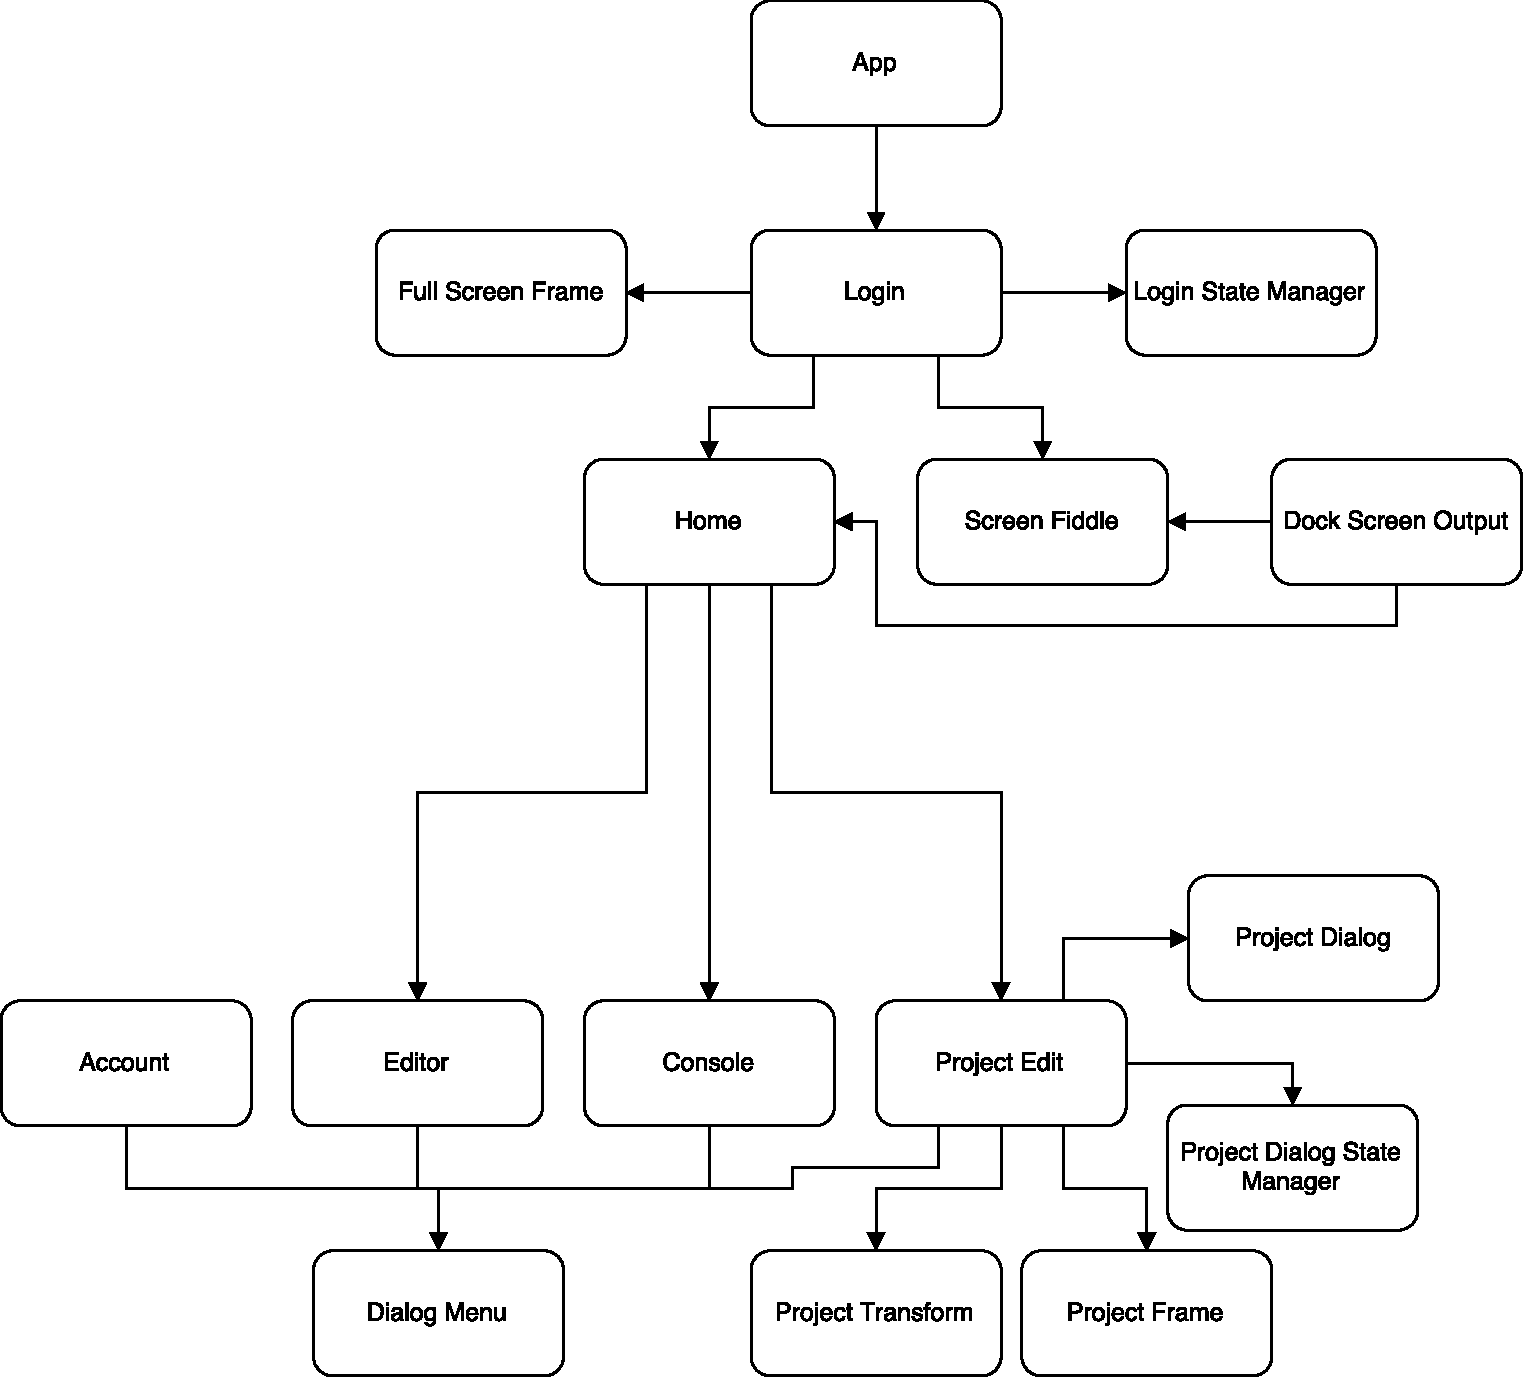
\includegraphics[width=0.7\textwidth]{uses-frontend.pdf}
\caption{Use hierarchy among front end modules}
\label{FigUH}
\end{figure}

\section*{Note}
The MIS documents do not include the front end UI modules since they're are not
server functions, methods and classes. They are essentially a markup of the UI
using JavaScript and the front end framework. Thus they are no included in the
MIS documents.

\section*{References}

\bibliographystyle {plainnat}
\bibliography {MG}

\end{document}
